%! TeX program = lualatex
%tags! intro first class digitales
\documentclass[letterpaper]{article}
\usepackage[margin=1in]{geometry}
\usepackage{amsmath}
\usepackage{amssymb}
\usepackage[no-math]{fontspec}
\usepackage[fg,bg]{gruvboxpalette}
\usepackage{hyperref}
\usepackage{newtxsf}
\usepackage[explicit]{titlesec}
\usepackage{tikz}
\usetikzlibrary{calc}
\usetikzlibrary{positioning}
\usetikzlibrary{arrows.meta}
\usepackage[most]{tcolorbox}
\usepackage{tabularray}
\DefTblrTemplate{firsthead, middlehead,lasthead}{default}{}
\DefTblrTemplate{capcont}{default}{}
\DefTblrTemplate{contfoot-text}{normal}{} \SetTblrTemplate{contfoot-text}{normal} \DefTblrTemplate{conthead-text}{normal}{} \SetTblrTemplate{conthead-text}{normal}
\UseTblrLibrary{counter}
\hypersetup{
  colorlinks  = true,
  urlcolor    = Blue,
  linkcolor   = Blue,
  citecolor   = Blue
}
\usepackage[most]{tcolorbox}

\setmainfont{NotoSans-Regular}[
Path           = /home/snouflake/.fonts/ ,
Extension      = .ttf ,
BoldFont       = NotoSans-Bold ,
ItalicFont     = NotoSans-Italic ,
BoldItalicFont = NotoSans-BoldItalic,
] 

\newtcolorbox{defbox}[3][]{%
  colback=blue!30!background,
  coltitle=blue!15!black,
  coltext=font,
  title filled=false,
	enhanced,
  detach title,
  tile,
  before upper={\tcbtitle\medskip\\},
  borderline west={2mm}{0pt}{blue},
  % attach boxed title to top center={yshift=-2mm},
  leftrule=2mm,
  toprule=0mm,
  bottomrule=0mm,
  rightrule=0mm,
  arc=0mm,
	title={Definición:~#2},
	#1
}

\setlength\parindent{0pt}

\usepackage{mathastext}

\def \T{Sistemas Digitales}
\def \S{2025-01-15}

\begin{document}
\begin{tikzpicture}[inner sep=0pt,color=font]
  \node[anchor=west,align=left,line width=0pt] 
    (title) at (0,0) {\huge\bfseries\noindent\T\\\Large\bfseries\S}
    ;
\end{tikzpicture}


\begin{longtblr}{
    colspec={@{}Q[3cm,cmd=\textbf,h] X@{}},
    rowsep={7pt}
  }
  Sistema digital
  & 
  Un sistema que utiliza numeros posicionales discretos
  \\
  Cambio de base
  & \begin{minipage}{\linewidth}
  \begin{center}
    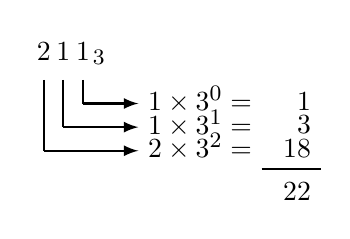
\begin{tikzpicture}[>=latex]
      \node (d3) at (0,0) {\strut2};
      \node[anchor=west] (d2) at ([xshift=-5pt] d3.east) {\strut1};
      \node[anchor=west] (d1) at ([xshift=-5pt] d2.east) {\strut1};
      \node[anchor=west,xshift=-6pt] (base) at (d1.east) {\strut$_{3}$};
      \coordinate (r) at (1.2,0);
      \draw[thick] (d1.south) to ($(d1.south) + (0,-0.3)$) coordinate (t1) edge[->] (t1-|r) coordinate (a1);
      \draw[thick] (d2.south) to ($(d2.south) + (0,-0.6)$) coordinate (t2) edge[->] (t2-|r) coordinate (a2);
      \draw[thick] (d3.south) to ($(d3.south) + (0,-0.9)$) coordinate (t3) edge[->] (t3-|r) coordinate (a3);
      \node[anchor=west] (math1) at (t1-|r) {\strut$1 \times 3^0 = $};
      \node[anchor=west] (math2) at (t2-|r) {\strut$1 \times 3^1 = $};
      \node[anchor=west] (math3) at (t3-|r) {\strut$2 \times 3^2 = $};
      \node[anchor=west,text width=0.5cm,align=right] (res1) at (math1.east) {\strut$1$};
      \node[anchor=west,text width=0.5cm,align=right] (res2) at (math2.east) {\strut$3$};
      \node[anchor=west,text width=0.5cm,align=right] (res3) at (math3.east) {\strut$18$};
      \draw[thick] ([yshift=3pt] res3.south west) -- ([yshift=3pt] res3.south east);
      \node[inner sep=0pt,anchor=north,text width=0.5cm,align=right]  at (res3.south) {\strut$22$};

    \end{tikzpicture}
  \end{center}
  \end{minipage}
  \\
  Alu
  & Arithmetic \& Logic Unit
  \\
  Complemento a la base
  & {
    $C_b(n) = b^{\text{\# of digits in n}} - n$

    $454_6 - 325_5 = 125$. $C_b(325) = 10_6^3 - 325_6 = 231_6$ 
    $454_6 + 231_6 = \text{\textcolor{blue}{1}}125$
    {\color{blue} si sobra un digito a la izquierda, se descarta y el resultado es positivo. Si no, el resultado es negativo y para obtener su magnitud, se le vuelve a sacar el complemento}
    \medskip

    {\bfseries{Esto pero en binario}}\\
    $C_b(n)$: De derecha izquierda ignorar todo hasta el primer 1 y luego voltear todo los bits. *Si el el minuendo tiene más digitos, se le añaden los 0 a la izquierda faltante al sustraendo.
  }
  \\
  Multiplicación
  & {
    $
    624_{7} \times 56_{7} =
    6 \times 4 \to ~_{7}
    + \left(6 \times 2 \to ~_{7}\right) \times 10_{7}
    + \left(6 \times 6 \to ~_{7}\right) \times 10_{7}^{2}
    + \left(
    5 \times 4 \to ~_{7}
    + \left(5 \times 2 \to ~_{7}\right) \times 10_{7}
    + \left(5 \times 6 \to ~_{7}\right) \times 10_{7}^{2}
    \right) \times 10_{7}^{2}
    $
  }
  \\
  División
  & {
    \begin{tabular}{rrrrr}
      0 & 1 & 2 & 3 & 4 \\
      0 & 4 & 13&22 &31 \\
    \end{tabular}

    \vspace{1cm}

    $231 \div 4 =$

    \begin{tblr}{colspec={r r l}}
      ~ &  31 & .22 \\
        \hline
      4 & 231 \\
        & 22~ \\
        \hline
        &   1 & 1 \\
      - &   4 \\
      \hline
        &   2 \\
      - &   1 & 3\\
      \hline
        &   0 & 2
    \end{tblr}
  }
  \\
  Conversión de base con división
  & {
    $325_6 \to ~_4 = 325_6 \div 4_6$
  }
\end{longtblr}


 
\end{document}
